% !TeX root = ../main.tex

\chapter{Marco Experimental y Datasets}

Este capítulo expone el marco metodológico y experimental  para la aplicación y evaluación de la arquitectura propuesta. En primer lugar, se describe el conjunto de datos empleado como base de aprendizaje del modelo, detallando el preprocesamiento del corpus masivo BIRD. A continuación, se define la cadena de procesamiento de la señal, centrada en el cálculo de la Curva de Decaimiento de Energía (EDC) para el correcto acondicionamiento y análisis de las respuestas acústicas. Finalmente, se detalla la fase de entrenamiento, estableciendo las estrategias de optimización y los criterios de evaluación que permiten cuantificar el rendimiento y la capacidad de generalización de la red neuronal.

\section{Corpus BIRD}

El \textit{Big Impulse Response Dataset} (BIRD) \cite{Grondin25} constituye la fuente principal de datos empleada en este trabajo para el entrenamiento y validación de la arquitectura DECOR. En su concepción original, este conjunto de datos se define como el mayor corpus abierto de respuestas al impulso en salas multicanal, compuesto por un total de 100.000 RIRs simuladas mediante el Método de la Imagen (\textit{Image Method}). Sin embargo, para los experimentos desarrollados en esta investigación, se ha seleccionado un subconjunto representativo de 40.000 respuestas. Esta dimensión muestral mantiene una base estadística suficientemente robusta para el entrenamiento de la red neuronal, a la vez que optimiza el coste computacional y los tiempos de iteración del modelo. 

El uso de este corpus presenta ventajas sustanciales para la tarea que nos ocupa. Cada simulación varía aleatoriamente parámetros clave como las dimensiones físicas de la sala, la velocidad del sonido y las posiciones relativas de 2 micrófonos y 4 fuentes de sonido omnidireccionales. Dado que el coste computacional espacial del Método de la Imagen escala de forma cúbica en el espacio tridimensional, disponer de un corpus precalculado de esta magnitud resulta fundamental para agilizar la experimentación.

\begin{figure}[htbp]
    \centering
    % Ajusta el valor 0.7 según lo grande que quieras que se vea en el PDF
    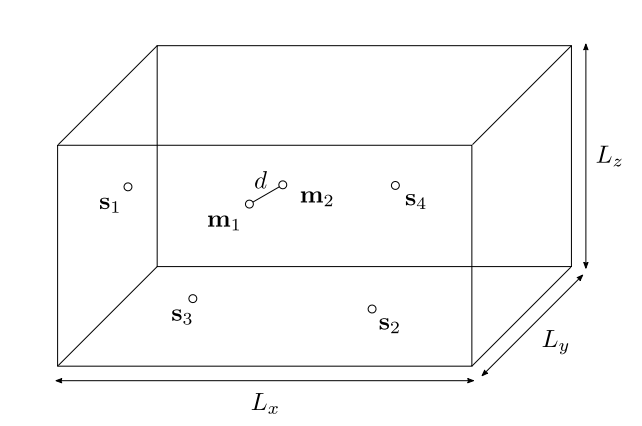
\includegraphics[width=0.7\textwidth]{Figures/bird.png}
    \caption[Configuración espacial BIRD]{Configuración espacial empleada para las simulaciones del corpus BIRD. El entorno virtual consiste en una sala rectangular de dimensiones $L_x \times L_y \times L_z$ metros, en la que se posicionan de manera aleatoria cuatro fuentes de sonido omnidireccionales ($\mathbf{s}_1, \mathbf{s}_2, \mathbf{s}_3, \mathbf{s}_4$) y un par de micrófonos ($\mathbf{m}_1, \mathbf{m}_2$) separados por una distancia $d$ \cite{Grondin25}.}
    \label{fig:bird_setup}
\end{figure}

No obstante, la utilización de BIRD para la extrapolación de la cola reverberante conlleva limitaciones inherentes a su naturaleza sintética que es crucial documentar. La topología del corpus representa una abstracción espacial simplificada: el algoritmo de simulación genera exclusivamente habitaciones vacías estrictamente rectangulares. En BIRD, la absorción de materiales no se modifica en sus RIRs: dentro de una misma sala se emplea un único coeficiente de absorción ($\alpha$) idéntico para todas las superficies (suelo, techo y paredes). 

Esta simplificación ignora la heterogeneidad de materiales presentes en entornos reales, lo que limita la variabilidad frecuencial y direccional de las reflexiones tardías que la red debe aprender a completar.  Desde el punto de vista operativo, los archivos de audio originales—generados a una frecuencia de muestreo nativa de 16 kHz y con 1 segundo exacto de duración (16.000 muestras)—son sometidos a una secuencia estricta de adecuación previa a su paso por la red neuronal. 

En primer lugar, cada señal multicanal se transforma a formato monoaural y se remuestrea a una frecuencia uniforme de 48 kHz, garantizando así la compatibilidad dimensional con la arquitectura DECOR. Sobre esta nueva base temporal, la respuesta se normaliza en amplitud y se alinea con respecto a su pico máximo para asegurar que el transitorio del sonido directo ocupe un índice determinista. Finalmente, la secuencia se ajusta a una longitud fija de 48.000 muestras (equivalentes a 1 segundo exacto).

Una vez acondicionada la señal, se procede a su segmentación en dos regiones de interés. Aprovechando la resolución obtenida tras el remuestreo, se aísla una cabeza temprana de longitud $N_{head} = 2400$ muestras (correspondientes exactamente a los primeros 50 ms), la cual abarca el sonido directo y las reflexiones tempranas. El resto de la secuencia conforma la cola reverberante remanente, que constituye el proceso de decaimiento tardío que el sistema debe aprender a extrapolar. 

\begin{figure}[htbp]
    \centering
    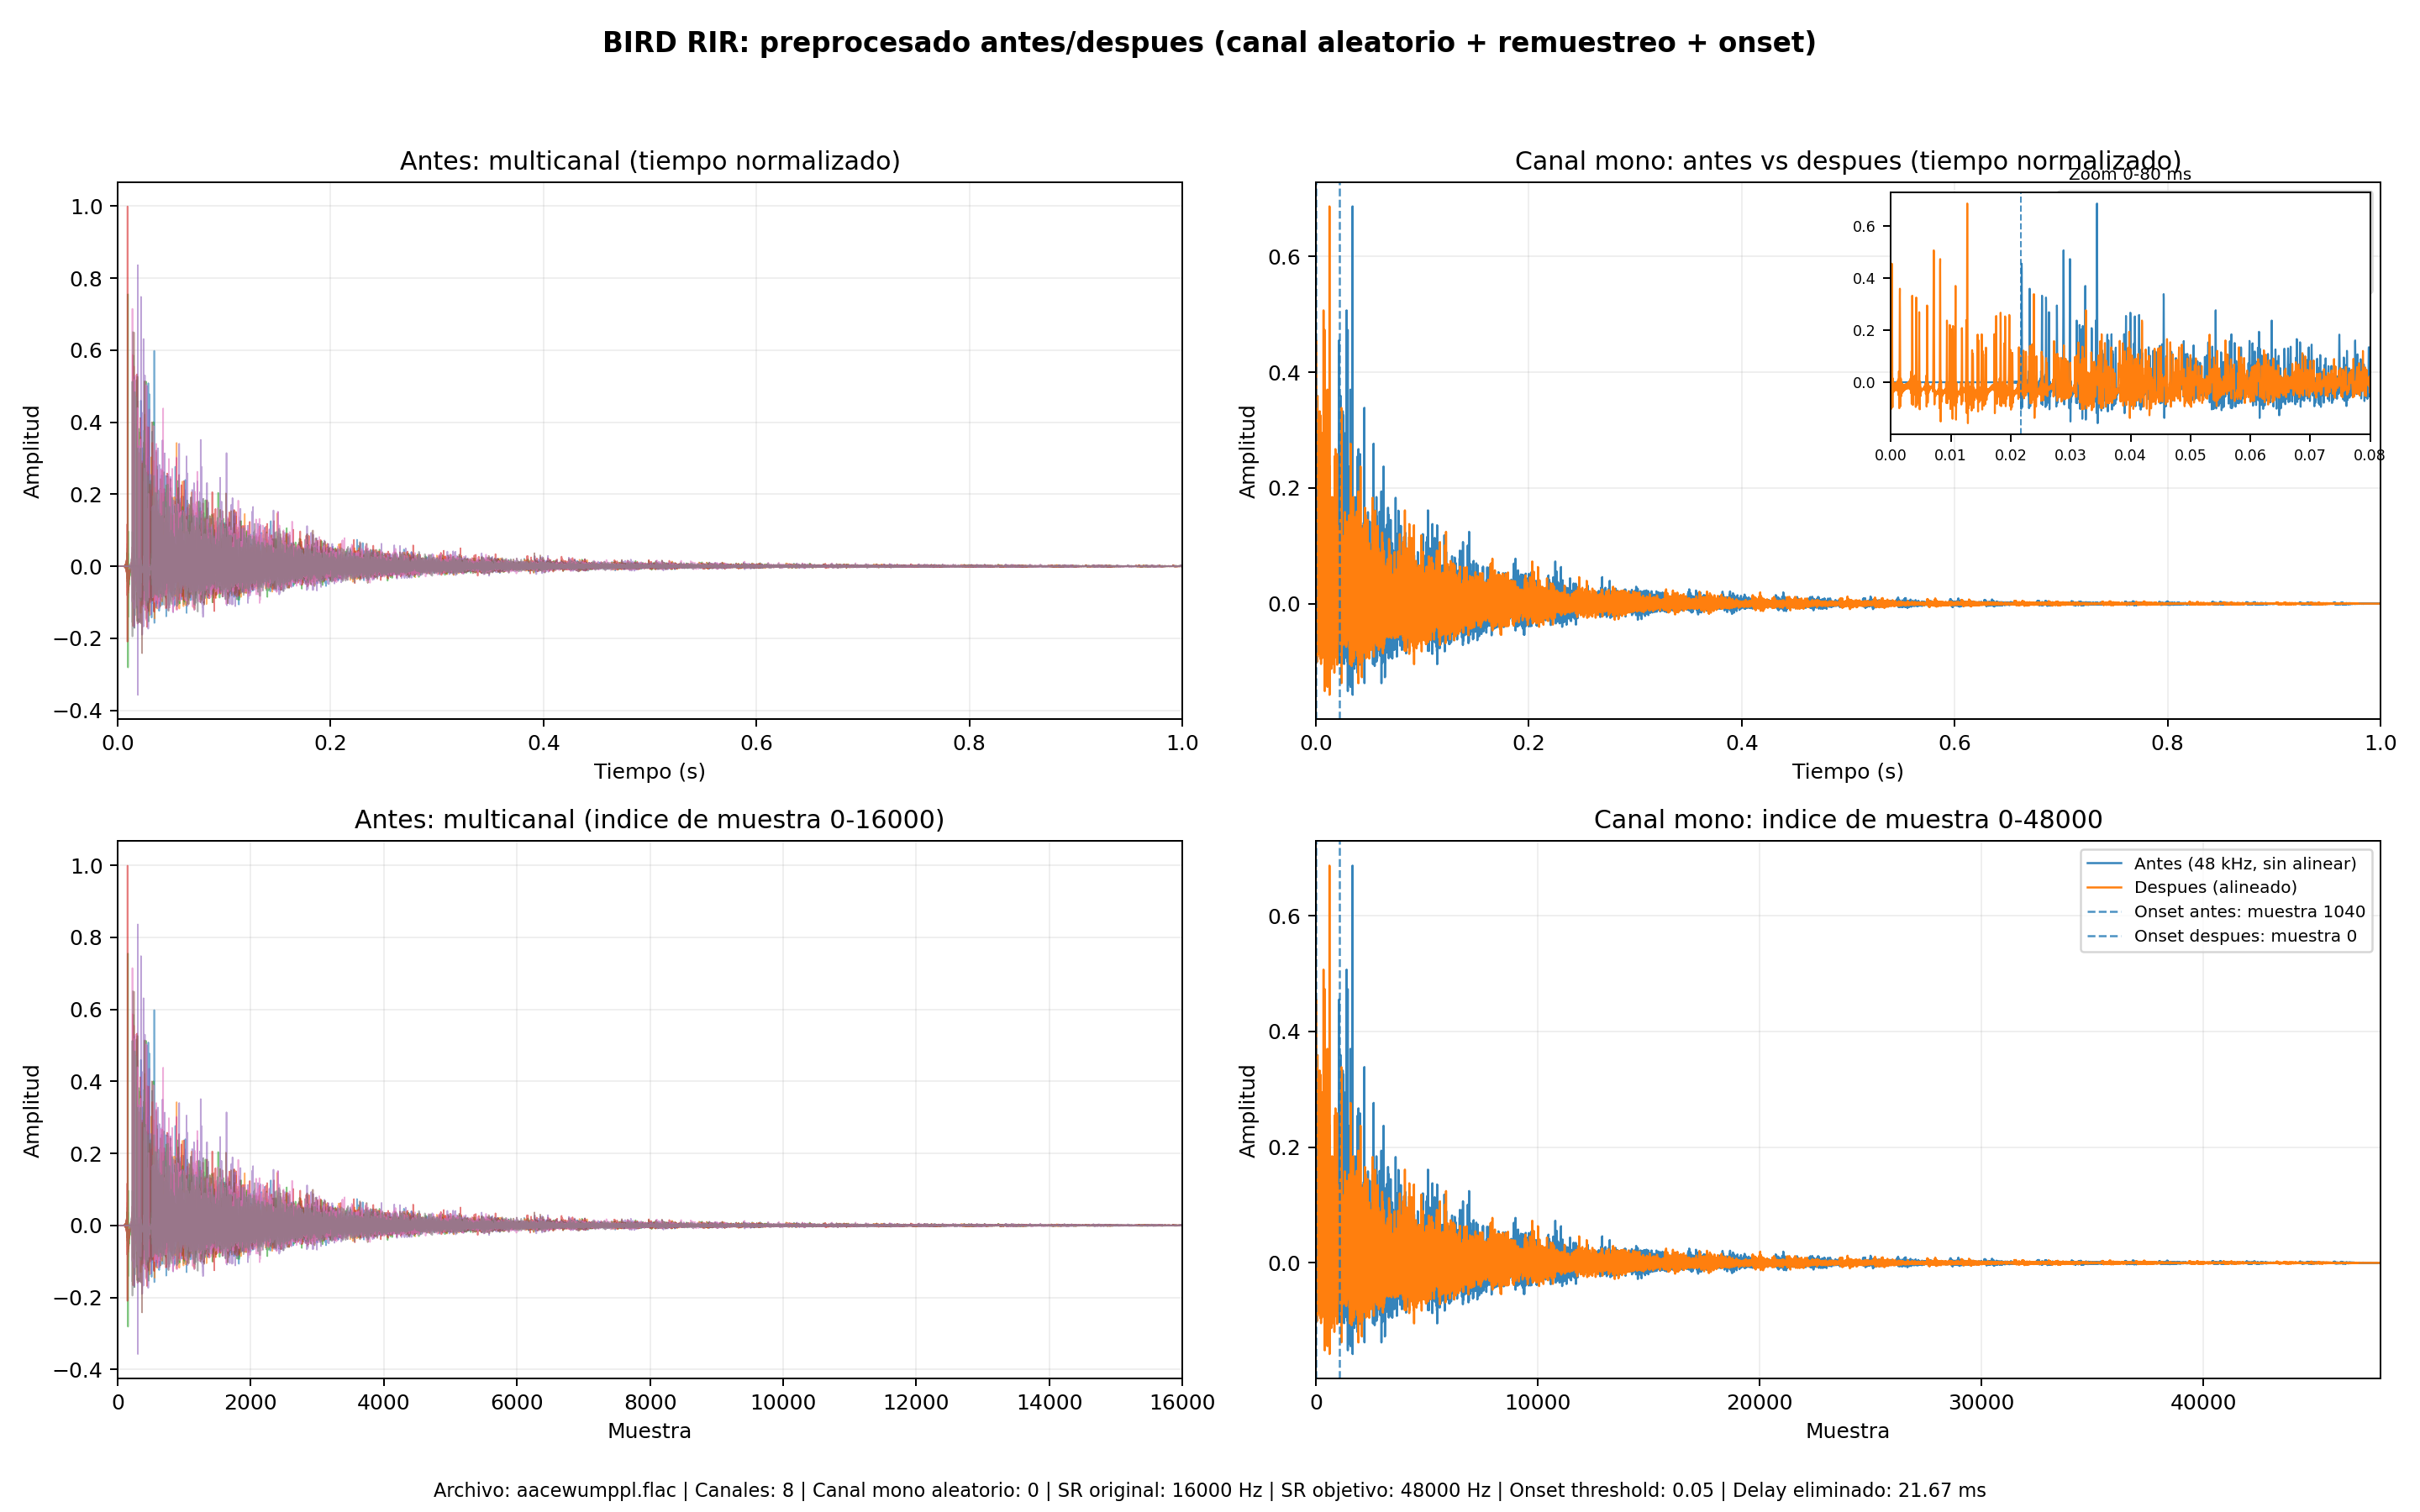
\includegraphics[width=1\textwidth]{Figures/bird_preprocess_before_after_onset.png}
    \caption[Preprocesado BIRD]{Efecto de la etapa de preprocesado sobre una respuesta al impulso del corpus BIRD. El procedimiento ilustrado incluye la extracción de un canal monoaural aleatorio, el sobremuestreo a 48 kHz y la alineación temporal basada en la detección de inicio (\textit{onset detection}). Este método elimina el tiempo de vuelo originado en la simulación preservando la integridad morfológica del sonido directo y de las reflexiones tempranas previas al pico de máxima amplitud.}
    \label{fig:bird_preprocessing_onset}
\end{figure}

Finalmente, para prevenir la contaminación cruzada y el solapamiento acústico, la división del subconjunto de 40.000 respuestas impulsionales entre las fases de entrenamiento y validación no se efectúa de manera aleatoria a nivel de impulso individual, sino aprovechando la estructura de bloques independientes (\textit{folds}) del corpus original. Al establecer la separación mediante estas agrupaciones de salas no solapadas, se garantiza que la evaluación se lleve a cabo sobre recintos acústicos no observados durante el ajuste de pesos, lo que proporciona una estimación rigurosa y fiable de la capacidad de generalización del modelo. 

En resumen, el corpus BIRD ofrece un entorno de simulación controlado y de gran escala para el entrenamiento de modelos de aprendizaje profundo en tareas de extrapolación temporal de RIR. Sin embargo, su naturaleza simulada y sus simplificaciones acústicas introducen limitaciones que deben ser consideradas al interpretar los resultados y extrapolar las conclusiones hacia escenarios del mundo real.

\section{Naive Baseline}

Para evaluar el rendimiento de nuestro modelo y entender el valor real de las métricas obtenidas, es fundamental contar con un punto de referencia básico o línea base. Con este propósito, implementamos un \textit{naive baseline} (o línea base ingenua), que consiste en una aproximación estocástica fija basada puramente en la media estadística del conjunto de datos.

\subsection*{Construcción de la Señal}
Este modelo de referencia no utiliza redes neuronales ni intenta extraer información de los primeros 50 ms del \textit{RIR head}. En su lugar, genera una única cola reverberante genérica combinando ruido blanco con una envolvente de decaimiento exponencial analítica. 

Los parámetros de esta señal (duración, energía y tiempo de reverberación) se configuran de forma estática utilizando los valores promedio de todo el conjunto de entrenamiento. Específicamente, se calibra para que coincida con el $T_{60}$ medio del \textit{dataset}, que en este trabajo es de 0.65 segundos. Posteriormente, esta misma señal fija se evalúa contra todos los RIR reales del conjunto de test para calcular sus métricas de error.

\subsection*{Formulación Matemática}
Matemáticamente, la señal del \textit{naive baseline} en el dominio temporal discreto se define mediante la siguiente ecuación:

\begin{equation}
    h_{\mathrm{naive}}(n) = w(n) \cdot e^{-\gamma n / f_s}
\end{equation}

Donde:
\begin{itemize}
    \item $h_{\mathrm{naive}}(n)$ es la respuesta al impulso calculada para la cola tardía.
    \item $w(n)$ es una secuencia de ruido blanco gaussiano que simula la densidad estocástica de las reflexiones.
    \item $f_s$ es la frecuencia de muestreo (en este trabajo, $f_s=48\,\mathrm{kHz}$).
    \item $\gamma$ es la tasa de decaimiento constante, la cual se vincula directamente al tiempo de reverberación promedio del conjunto de datos ($T_{60,\mathrm{mean}} = 0.65$ s) mediante la relación de atenuación de 60 dB:
    \begin{equation}
        \gamma = \frac{\ln(10^3)}{T_{60,\mathrm{mean}}} \approx \frac{6.91}{T_{60,\mathrm{mean}}}
    \end{equation}
\end{itemize}

\subsection*{Utilidad y Justificación en el Trabajo}
La inclusión de este caso de control es importante en el empleo de nuestro trabajo por tres motivos principales:

\begin{enumerate}
    \item \textbf{Establecer un límite inferior :} Nos da el peor escenario aceptable. Cualquier modelo de aprendizaje profundo que diseñemos debe superar  los resultados de esta aproximación matemática simple para justificar su complejidad computacional.
    \item \textbf{Validar el comportamiento de la red:} Si el modelo DECOR obtiene errores significativamente menores que el \textit{naive baseline}, queda demostrado estadísticamente que la red no se está limitando a devolver la media estocástica de las salas que ha visto durante el entrenamiento, sino que extrae características acústicas específicas del \textit{head} de 50 ms.
    \item \textbf{Contextualizar la escala de los errores:} Nos ayuda a interpretar físicamente las magnitudes de evaluación. Al comparar nuestros resultados frente a la desviación de la media, podemos cuantificar con precisión el porcentaje de mejora del sistema propuesto.
\end{enumerate}
\section{Pipeline EDC}

Dentro del flujo de procesamiento de datos, el cálculo de la Curva de Decaimiento de Energía (EDC, por sus siglas en inglés) se establece como métrica fundamental para evaluar la coherencia del decaimiento reverberante. Dado que la respuesta al impulso tardía presenta un comportamiento altamente estocástico, resulta inviable predecir su forma de onda exacta. Por ello, la EDC permite extraer una envolvente energética determinista que el modelo sí puede aprender a extrapolar. Para una secuencia discreta de la cola reverberante $y[n]$ de longitud $N$, se emplea la forma de integración discreta propuesta originalmente por Schroeder \cite{Schroeder1965}:

\begin{equation}
\mathrm{EDC}_{norm}[t] = \frac{\sum_{n=t}^{N-1} y[n]^2}{\sum_{n=0}^{N-1} y[n]^2}
\end{equation}

En esta formulación, donde $y[n]$ representa la secuencia discreta de la cola reverberante, la EDC se normaliza por la energía total de la cola para garantizar que su valor inicial sea exactamente 1 (0 dB) y que tienda asintóticamente a 0 a medida que el tiempo avanza. Esta normalización es crucial para establecer una escala de análisis coherente y para facilitar la comparación entre diferentes muestras con niveles de energía variables, garantizando una trayectoria monótona decreciente acotada en el intervalo $[0,1]$, con valor unitario al inicio del decaimiento y aproximación asintótica a cero para tiempos tardíos.

Con el fin de obtener una escala de análisis perceptualmente adecuada, la curva normalizada se expresa en decibelios mediante transformación logarítmica:

\begin{equation}
\mathrm{EDC}_{dB}[t] = 10 \log_{10}\left( \max(\mathrm{EDC}_{norm}[t], \epsilon) \right)
\end{equation}

\begin{figure}[htbp]
    \centering
    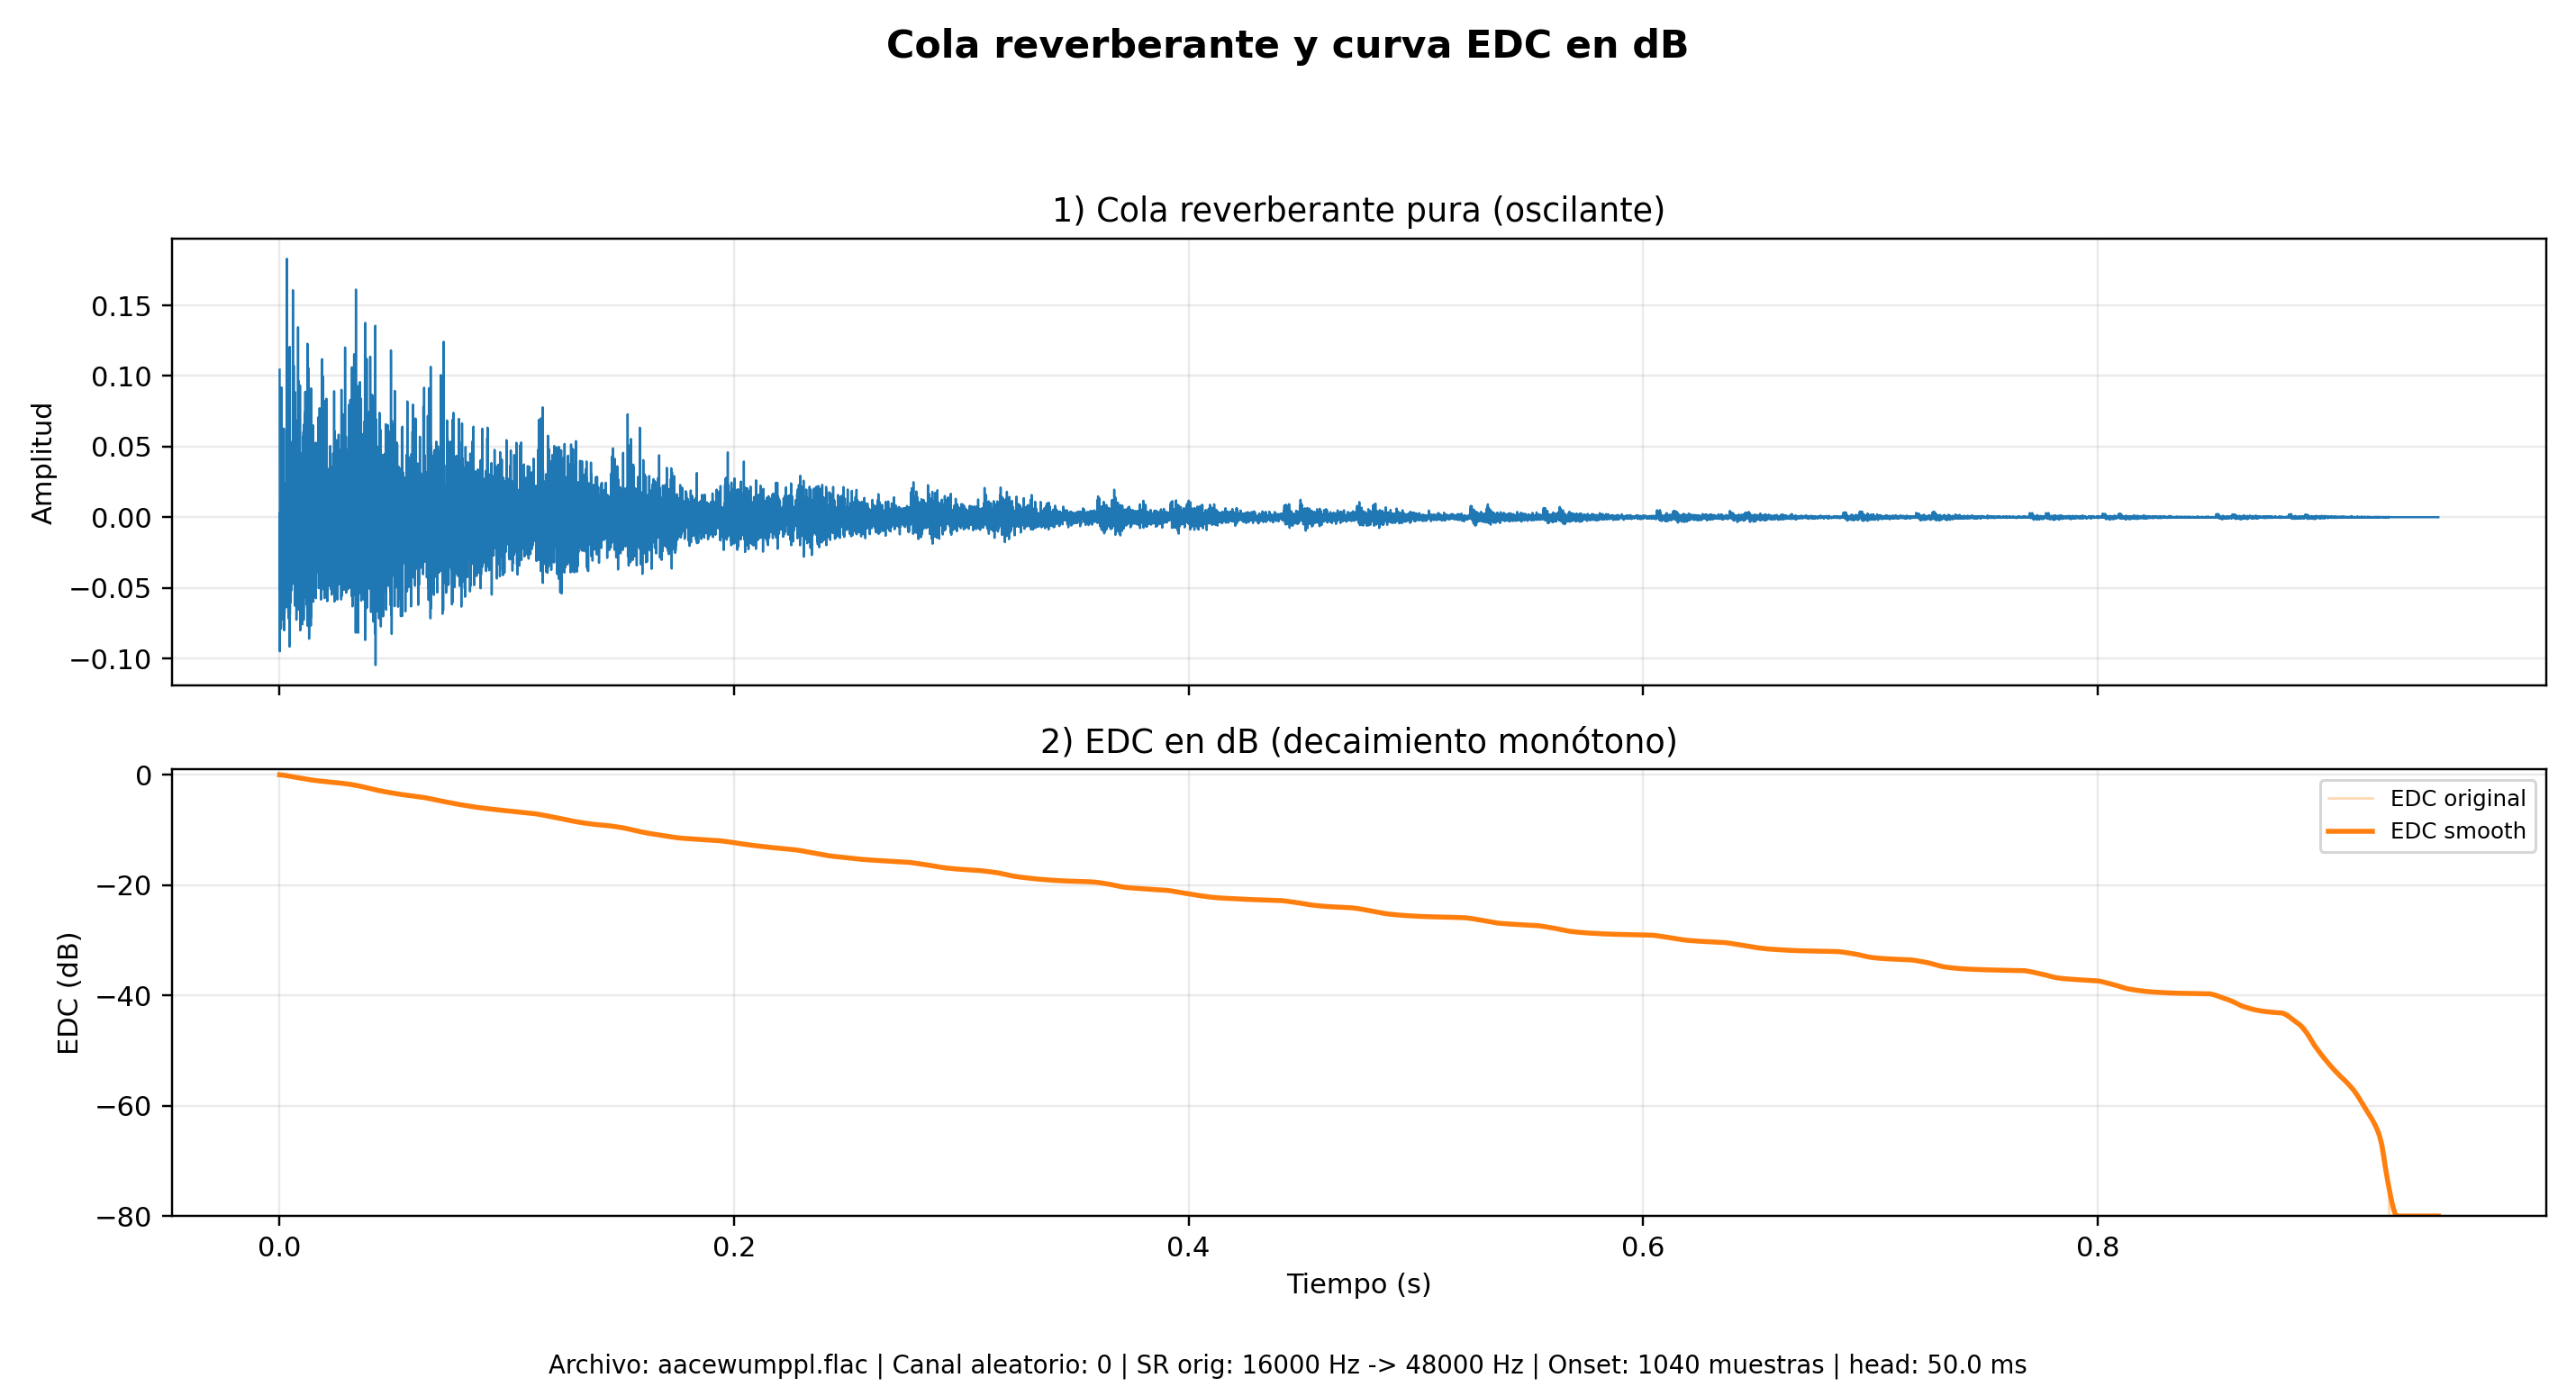
\includegraphics[width=0.8\textwidth]{Figures/tail_edc_overlay.png}
    \caption[Curva de Decaimiento de Energía (EDC) ]{Comparativa visual entre la forma de onda estocástica de una cola reverberante y su correspondiente Curva de Decaimiento de Energía (EDC) expresada en decibelios. Se observa cómo la integración de Schroeder extrae una envolvente energética determinista y monótonamente decreciente, transformando la señal bruta en un objetivo de aprendizaje estable para el modelo predictivo.}
    \label{fig:edc_schroeder}
\end{figure} 

El término de protección $\epsilon$, asociado en práctica a un suelo dinámico del orden de -80 dB, resulta indispensable para preservar estabilidad numérica en el cálculo tensorial, evitando singularidades cuando la energía remanente tiende a cero.

Desde la perspectiva computacional, la lógica de segmentación temporal (corte exacto en la muestra 2400) y el cálculo de la EDC se implementan dentro de estructuras de carga iterativa (\textit{DataLoaders}). Esto permite generar tensores de manera dinámica y empaquetarlos en lotes (\textit{batches}), manteniendo un flujo de memoria estable hacia GPU sin colapso de memoria principal. De forma simultánea, se conserva la trazabilidad exacta entre la cabeza de entrada, la cola objetivo y su EDC analítica en cada muestra procesada.

\section{Entrenamiento}

La fase de entrenamiento de la red neuronal se llevó a cabo utilizando el entorno basado en la nube Google Colab Pro, haciendo uso de una GPU NVIDIA A100. Las prestaciones de esta unidad de procesamiento gráfico resultan plenamente adecuadas para satisfacer la demanda computacional del modelo, permitiendo gestionar de manera eficiente las  secuencias temporales inherentes al procesamiento de audio.
 La adopción de esta infraestructura basada en la nube destaca por ofrecer acceso inmediato a \textit{hardware} de alto rendimiento sin requerir una elevada inversión en equipamiento local. No obstante, este entorno introduce limitaciones operativas significativas, tales como la interrupción forzosa de las sesiones por límites de tiempo y la dependencia de sistemas de almacenamiento no persistentes. En consecuencia, el uso de esta plataforma exigió la implementación de rutinas de guardado periódico (\textit{checkpoints}) para salvaguardar los pesos de la red y mitigar la volatilidad del sistema.

Para garantizar la solidez de la evaluación ante datos no observados, se adoptó una estrategia de validación cruzada (\textit{k-fold cross-validation}). El corpus se dividió manteniendo una proporción estricta de 3 \textit{folds} dedicados a la fase de aprendizaje por cada \textit{fold} reservado para la evaluación del rendimiento. Esta metodología asegura que el modelo se ajuste a una variedad de escenarios acústicos durante el entrenamiento, mientras que la validación se realiza sobre recintos completamente nuevos, lo que proporciona una estimación rigurosa de la capacidad de generalización del sistema.

Por otro lado, para dirigir el aprendizaje del modelo hacia una solución que sea tanto acústicamente precisa como físicamente coherente, la dinámica de ajuste de parámetros no puede depender de un único criterio. En su lugar, se rige por una función de coste compuesta que equilibra la fidelidad espectral y el comportamiento temporal del sonido: 

\begin{equation}
\mathcal{L}_{total} = \lambda_{\mathrm{MSTFT}} \cdot \mathcal{L}_{MSTFT} + \lambda_{\mathrm{EDC}} \cdot \mathcal{L}_{EDC-L1}
\end{equation}

Esta formulación combina el error espectral multiresolución, ponderado por $\lambda_{\mathrm{MSTFT}}$, con el error absoluto asociado a la curva de decaimiento energético temporal, ponderado por $\lambda_{\mathrm{EDC}}$. Dentro del protocolo de validación, la métrica $L1$ sobre la EDC se establece como indicador principal para verificar la precisión física de la respuesta sintetizada durante el ciclo iterativo de aprendizaje.

Por último, la actualización de pesos se emplea con \textbf{Ranger21} \cite{Ranger21}, un optimizador diseñado para ejecutar trayectorias de aprendizaje prolongadas de forma robusta. Su elección se justifica por la incorporación de mecanismos de estabilización fundamentales para este tipo de modelado:
\begin{itemize}
    \item \textbf{Recorte de gradientes (\textit{Gradient Clipping}):} Permite mitigar el riesgo de explosión de gradientes, una inestabilidad característica cuando se trabaja en la predicción de secuencias largas.
    \item \textbf{Fase de enfriamiento (\textit{Cooldown}):} Consiste en una reducción progresiva de la tasa de aprendizaje durante las últimas épocas del entrenamiento, lo que favorece una aproximación estable hacia mínimos más profundos en la superficie de coste.
\end{itemize}


El protocolo de entrenamiento se estructura en tres fases claramente diferenciadas:
\begin{enumerate}
\item \textbf{Fase 1 (Épocas 1 a 20) --- Inicialización Frecuencial.}
El entrenamiento se inició con un tamaño de lote de 128 muestras y una tasa de aprendizaje de $1\cdot 10^{-4}$. En esta etapa se establecieron los pesos de la función de coste como $\lambda_{\mathrm{EDC}}=0.0$ y $\lambda_{\mathrm{MSTFT}}=1.0$. El propósito consistió en permitir que la red asimilara la estructura espectral de la cola reverberante sin imponer todavía penalización temporal explícita, favoreciendo un asentamiento inicial de los parámetros del decodificador. Al cierre de esta fase se obtuvo una pérdida de validación (Val Loss) de 11.13 y un error EDC-L1 preliminar de 0.10.

\begin{lstlisting}[style=pythoncell,caption={Ejecución de entrenamiento correspondiente a la Fase 1.},label={lst:fase1_train}]
DATA_LOCAL="/content/BIRD_Local"
CHECKPOINT_DRIVE="/content/drive/MyDrive/BIRD_Dataset/decor_best_model.pth"

!python scripts/train.py \
	--data-root "$DATA_LOCAL" \
	--epochs 20 \
	--batch-size 128 \
	--lr 1e-4 \
	--num-workers 8 \
	--checkpoint "$CHECKPOINT_DRIVE"
\end{lstlisting}

\item \textbf{Fase 2 (Épocas 21 a 400) --- Estabilización Transitoria y Acoplamiento Físico.}
La transición hacia la optimización conjunta mostró una inestabilidad intensa cuando se activó de forma abrupta la penalización temporal con $\lambda_{\mathrm{EDC}}=0.1$, observándose explosión de la norma del gradiente y aumento de la pérdida por encima de 19. Para mitigar este comportamiento se aplicó una estrategia progresiva: la tasa de aprendizaje se redujo a $1\cdot 10^{-5}$ y el término temporal se suavizó inicialmente a $\lambda_{\mathrm{EDC}}=0.01$, elevándolo de manera gradual hasta $\lambda_{\mathrm{EDC}}=0.05$. De forma complementaria, el tamaño de lote se amplió a 256 muestras para aprovechar la capacidad de cómputo de los aceleradores gráficos y disminuir la varianza estocástica del gradiente. Bajo este esquema el optimizador absorbió la nueva restricción y, en la época 390, se superó la barrera de pérdida con una Val Loss de 9.41 y un error EDC-L1 de 0.085.

\begin{lstlisting}[style=pythoncell,caption={Ejecución de entrenamiento correspondiente a la Fase 2.},label={lst:fase2_train}]
!python scripts/train.py \
    --data-root "$DATA_LOCAL" \
    --epochs 400 \
    --batch-size 256 \
    --lr 1e-5 \
    --loss-alpha 0.05 \
    --loss-beta 1.0 \
    --num-workers 8 \
    --resume "$CHECKPOINT_PREVIO" \
    --checkpoint "$NUEVO_CHECKPOINT"
\end{lstlisting}

\item \textbf{Fase 3 (Épocas 401 a 590) --- Afinación Fina y Convergencia Asintótica.}
En la etapa final se mantuvieron fijos el tamaño de lote en 256 y el peso temporal en $\lambda_{\mathrm{EDC}}=0.05$, operando con una tasa de aprendizaje conservadora de $1\cdot 10^{-5}$ para recorrer el entorno del mínimo con mayor precisión. La fase de enfriamiento (\textit{Cooldown}) de Ranger21 resultó determinante en este tramo, promoviendo el asentamiento definitivo de los pesos y una convergencia estable. En la iteración terminal se extrajo el punto de control óptimo (\textit{checkpoint}), registrándose un mínimo absoluto histórico con Val Loss de 9.345, resultado que respalda la eficacia del protocolo de entrenamiento.

\begin{lstlisting}[style=pythoncell,caption={Ejecución de entrenamiento correspondiente a la Fase 3 (pulido final).},label={lst:fase3_train}]
!python scripts/train.py \
	--data-root "$DATA_LOCAL" \
	--epochs 590 \
	--batch-size 256 \
	--lr 1e-5 \
	--loss-alpha 0.05 \
	--loss-beta 1.0 \
	--num-workers 8 \
	--resume "$CHECKPOINT_PREVIO" \
	--checkpoint "$NUEVO_CHECKPOINT"
\end{lstlisting}
\end{enumerate}

\section{Métricas de Evaluación}

Se utilizan cuatro métricas objetivas para evaluar el rendimiento de los modelos: el error de MSTFT, el error de la función de decaimiento de la energía (EDF), el error del tiempo de reverberación ($T_{60}$) y el error de la relación sonido directo-reverberante (DRR). Estas métricas ofrecen una indicación aproximada de la capacidad para igualar las características acústicas de la sala objetivo.

El error de MSTFT evalúa la similitud de dos espectros RIR en múltiples resoluciones STFT. Además de utilizarse como función de pérdida durante la fase de entrenamiento, sigue siendo útil como métrica de evaluación, ya que tiene en cuenta las diferencias espectrales y temporales en el dominio STFT. 

El error EDF es el error entre la EDF predicha y la real \cite{Steinmetz2021FiNS}. El modelo se evalúa utilizando el error absoluto medio (MAE) y la raíz del error cuadrático medio (RMSE).

\begin{equation}
\mathcal{L}_{\mathrm{EDF,\,MAE}} = \frac{1}{T} \sum_{n=1}^{T} \left| \hat{d}^{(\mathrm{dB})}[n] - d^{(\mathrm{dB})}[n] \right|
\end{equation}

\begin{equation}
\mathcal{L}_{\mathrm{EDF,\,RMSE}} = \sqrt{\frac{1}{T} \sum_{n=1}^{T} \left[ \hat{d}^{(\mathrm{dB})}[n] - d^{(\mathrm{dB})}[n] \right]^2}
\end{equation}

donde las EDF $\hat{d}^{(\mathrm{dB})}[n]$ y $d^{(\mathrm{dB})}[n]$ se calculan mediante la integral de Schroeder \cite{Schroeder1965} y se representan en una escala logarítmica en dB. El error EDF cuantifica cuánto difiere el decaimiento de la energía sonora entre la RIR real y la predicha.

Por otro lado, el error $T_{60}$ es una métrica ampliamente utilizada para evaluar la generación de reverberación, ya que captura de manera general la similitud en el tiempo de reverberación, el cual es un indicio perceptual del tamaño de la sala y la absorción acústica. El error $T_{60}$ es el error porcentual absoluto medio (MAPE) entre el tiempo de reverberación real $T_{60,c}$ y el predicho $\widehat{T}_{60,c}$ a lo largo de $n$ bandas de octava, es decir,

\begin{equation}
\mathrm{T}_{60,\mathrm{MAPE}} = 100 \frac{1}{n} \sum_{c=1}^{n} \left| \frac{\widehat{T}_{60,c} - T_{60,c}}{T_{60,c}} \right|
\end{equation}

Los valores de $T_{60}$ correspondientes a las RIR de referencia y generadas se estimaron utilizando DecayFitNet, una herramienta introducida por \cite{EDF22} que permite una estimación del $T_{60}$ robusta frente al ruido de fondo de la cola estocástica. Dicho análisis abarca las bandas de octava cuyas frecuencias centrales se sitúan en $f_c = \{125, 250, 500, 1000, 2000, 4000\}$.

La última métrica importante para evaluar el modelo es el error DRR, que es el MSE entre la RIR real y la predicha. El DRR es un ratio de energía, formado por la energía del sonido directo dividida por la energía de la reverberación tardía. Se calcula como: 

\begin{equation}
\mathrm{DRR} = 10 \log_{10} \left( \frac{\sum_{n=n_d-n_0}^{n_d+n_0} h[n]^2}{\sum_{n=n_d+n_0}^{N-1} h[n]^2} \right)
\end{equation}     

donde $n_d$ es el índice de la muestra del pico del sonido directo, $n_0$ es el número de muestras correspondientes a 1 ms de tiempo (es decir, $n_0 = 48$ muestras para $f_s = 48$ kHz), y $N$ es la longitud total de la RIR discreta. 

Para evaluar las métricas de $T_{60}$ y DRR, se emplea un conjunto de 1000 RIRs de prueba que no se han utilizado durante el entrenamiento. Este conjunto de prueba se selecciona de manera que las salas representadas no se solapen con las utilizadas en la fase de entrenamiento, garantizando así una evaluación objetiva y representativa del rendimiento del modelo en entornos acústicos no vistos previamente. Así verificamos la capacidad de generalización del modelo y su eficacia en la extrapolación de la cola reverberante en escenarios acústicos diversos. Como demuestran Lin et al. \cite{Lin25}, la arquitectura DECOR conserva la capacidad de extrapolar la cola reverberante incluso en salas no vistas durante el entrenamiento, aunque lo hace de manera menos precisa.